% Chapter 5

\chapter{Desarrollo Practicas} % Main chapter title

\label{Chapter5} % For referencing the chapter elsewhere, use \ref{Chapter1} 

% -------------------------------------------------------------------------------------------
% Practica PACMAN
%------------------------------------------------------------------------------------------
\section{Pac-man}
Se quiere implementar tecnología del lado del cliente como punto de partida en este curso. Se
quiere que se coja soltura en el manejo de eventos y programación con JavaScript que será donde
mayor peso tenga la práctica.
Como complemento se utilizará HTML5 enfocándonos en las novedades que presenta como la
etiqueta canvas y audio mientras y la API de LocalStorage.
\subsection{Un poco de historia}
\begin{wrapfigure}{l}{0.35\textwidth}
  \begin{center}
    
\includegraphics[width=0.4\textwidth]{Figures/pac_man}
      \end{center}
\end{wrapfigure}
En el año 1980, en los salones recreativos de Japón destacaban los juegos shoot 'em up, como
por ejemplo Space Indevaders, dirigido principalmente al género masculino
Es cuando Toru Iwatani, diseñador Namco, decide crear un juego que rompa con la tendencia del
momento además quería quitar la orientación de los videojuegos hacia el género masculino.
La idea surgió cuando Toru Iwatani estaba comiendo un trozo de pizza y al quitar un trozo
apareció la forma del que se convertiría en Pacman. El nombre original de Pacman es Paku-Paku
(que en japonés significa comer).
El 22 de mayo del mismo año fue instalado en las máquinas recreativas de Japón, el cual tuvo un
éxito comercial que sus creadores no hubiesen imaginado. No fue hasta cinco meses más tarde que
llegaría a Estados Unidos donde se le cambio el nombre por Pacman.
\subsection{Técnicas de implementación}
\subsubsection{Canvas}
Es la base de nuestra aplicacion  ya que como se comento en point.3 nos permite trabajar con elementos graficos dentro del navegador.
Dispone de diferenteste elementos que facilitan realizar dibujos sobre el lienzo a continuacion explicaremos los elementos que se van a utilizar para el desarrollo de la practica.
\begin{enumerate}
\item \textbf{2d Context}\\ A traves de la etiqueta canvas accedemos al contexto del elemento , en nuestro caso se trata de un contexto en 2d ya que utilizamos  imagenes y elementos planos aunque soporta tambien el contexto 3d.\\Dispone de dos metodos uno para guardar el estado actual del dibujar 'save()' y el otro recupera el estado guardado  'restore()'
\item \textbf{Imagenes}\\ Para trabajar con imagenes dispones del metodo ‘drawImage()’ .Este metodo se encuentra sobrecargado, es decir, segun el numero de parametros  trabaja de diferente forma con la imagen.\\ Con respecto a la practica se trabaja con imagenes normales y spreedsheet , a continuacion explicamos el enfoque en cada caso .
\begin{itemize}
\item Sprite sheet :  conjunto de pequeñas imagenes dentro de un imagen general,cada pequeña imagen tiene el mismo ancho y largo. Lo utilizamos para dibujar a Pacman,Fantamas y frutas del juego por lo que la llamada al metodo es  'drawImage(img,sx,sy,sw,sh,dx,dy,dw,dh)' .\\ La accion que realizara es cortar una seccion de la imagen original y colocarla en un punto del lienzo con unas determinadas dimensiones.\begin{figure}[h]
\begin{center}
   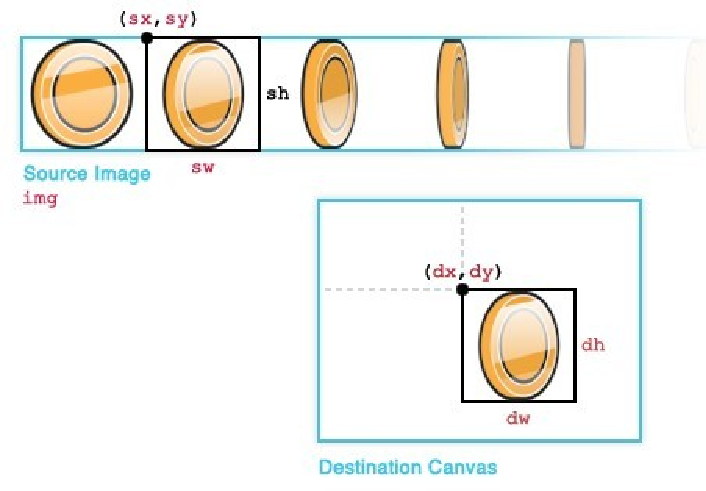
\includegraphics[width=0.5\linewidth, height=5cm]{Figures/SpreedSheet}
	\decoRule
	\caption[Contorno Escenario]{Contorno Escenario.}
\label{fig:canvasPrimitivas}
\end{center}\end{figure}
\item Imagenes:a difertencia del caso anterior cargamos la imagen directamente sin modificar su aspecto realizando la llamada al metodo  como 'drawImage(img,x,y)' 
\end{itemize}

\item \textbf{Texto}\\Podemos generar cualquier tipo de caracter para representa informacion dentro  de canvas .\\En nuestra practica lo utilizamos para informarmar al usuario de sus puntuacion,numero de vidas y el cronometro.
\item \textbf{Path}\\Nos permite trabajar con un conjunto de  primitivas basicas que son accesibles a traves del contexto del elemento.\\Pasamos a explicar los elementos empleados en la practica. 
\begin{itemize}
\item beginPath() / closePath() : metodos que marcan el inicio y el final de los elementos que foman el dibujo que se necesite realizar. \ref{fig:canvasPrimitivas}
\item moveTo(x,y): permite moverse a un punto del lienzo para empezar a dibujar a partir de el. \ref{fig:canvasPrimitivas}
\item lineTo(x,y):a traves de este metodo podemos  dibujar una linea.Toma como punto de partida el ultimo punto conocido y como  punto final  la coordenada que se le pasa . \ref{fig:canvasPrimitivas} \begin{figure}[h]
\begin{center}
   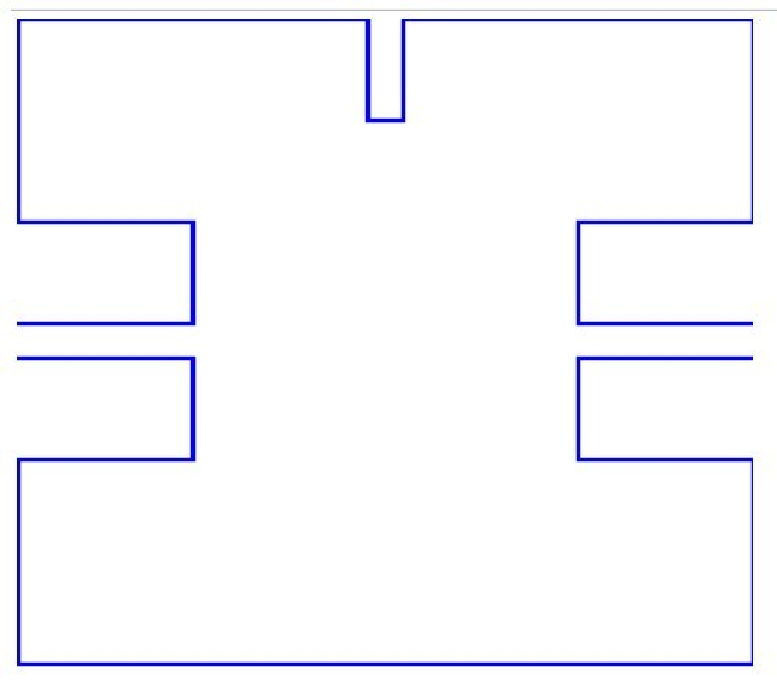
\includegraphics[width=0.4\linewidth, height=5cm]{Figures/canvasPrimitivas}
	\decoRule
	\caption[Contorno Escenario]{Contorno Escenario.}
\label{fig:canvasPrimitivas}
\end{center}
\end{figure} 
\item rect(x,y,width,heigth): permite dibujar un rectangulo con los parametro que se le pasa al metodo dentro del lienzo.\ref{fig:canvasCirc}
\item arc(x,y,radio,angInit,angFin,true): permite dibujar circunferencia,medias circunferenica. Para realizar este proceso establece como centro las coordenadas (x,y) ,su tamaño depened del radio que se especique y por ultimo establemos el angulo inical y final que queremos.\ref{fig:canvasCirc}  \begin{figure}[h]
\begin{center}
   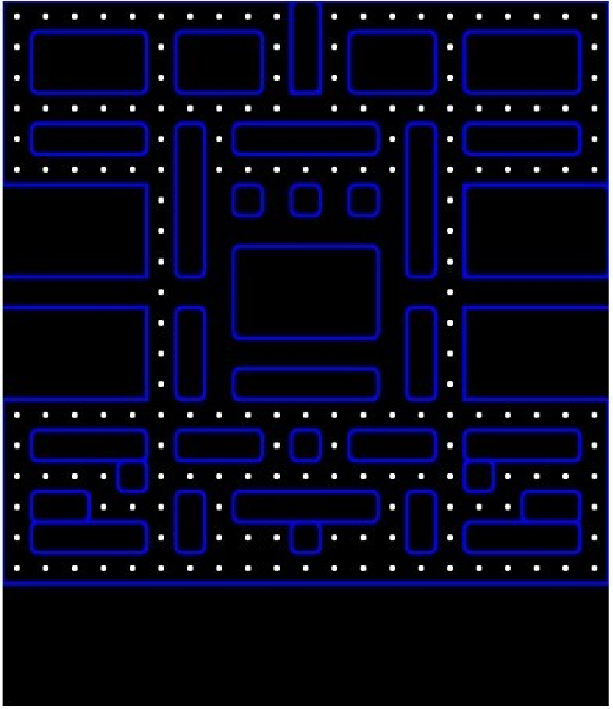
\includegraphics[width=0.5\linewidth, height=8cm]{Figures/canvasCirc}
	\decoRule
	\caption[An Electron]{An electron (artist's impression).}
\label{fig:canvasCirc}
\end{center}
\end{figure}  
\end{itemize}
\end{enumerate}
\subsubsection{Inteligencia Artificial (Dijkstra)}
Se necesita dar  autonomia a los fantasmas del juego por lo que es necesario utilizar un algoritmo que les permita conocer el camino a seguir hasta su objetivo. Existen varios script que implementan el funcionamiento dentro de todos estos hemos seleccionado 'astar.js'\\
El algoritmo utiliza el Teorema Dijkstra que permite calcular la distancia que existe entre los distintos nodos que forman el grafo de trabajo y selecciona el más corto.Para emplerar el algoritmo tenemos necesitamos los siguientes elementos.\\
Necesitamos crear una matriz bidimensional que representa el escenario del juego.Esta matriz tiene dos posibles valores el '0' que representa un obstaculo por lo que no es un punto accesible mientras que el valor '1' es un punto accesible.\\
Ahora aplicamos el script 'astar.js' para generar el grafo con la funcion 'Grap(matriz)'  a partir de este elemento seleccionamos  nodo inicial y final  a traves de la funcion ‘Graph.grid[x][y]’. Finalmente,pasamos a calcular la lista de nodos con la funcion 'search (pInicial, pFinal,false)‘. \ref{fig:InteligenciaArtificial}   
 \begin{figure}[h]
\begin{center}
   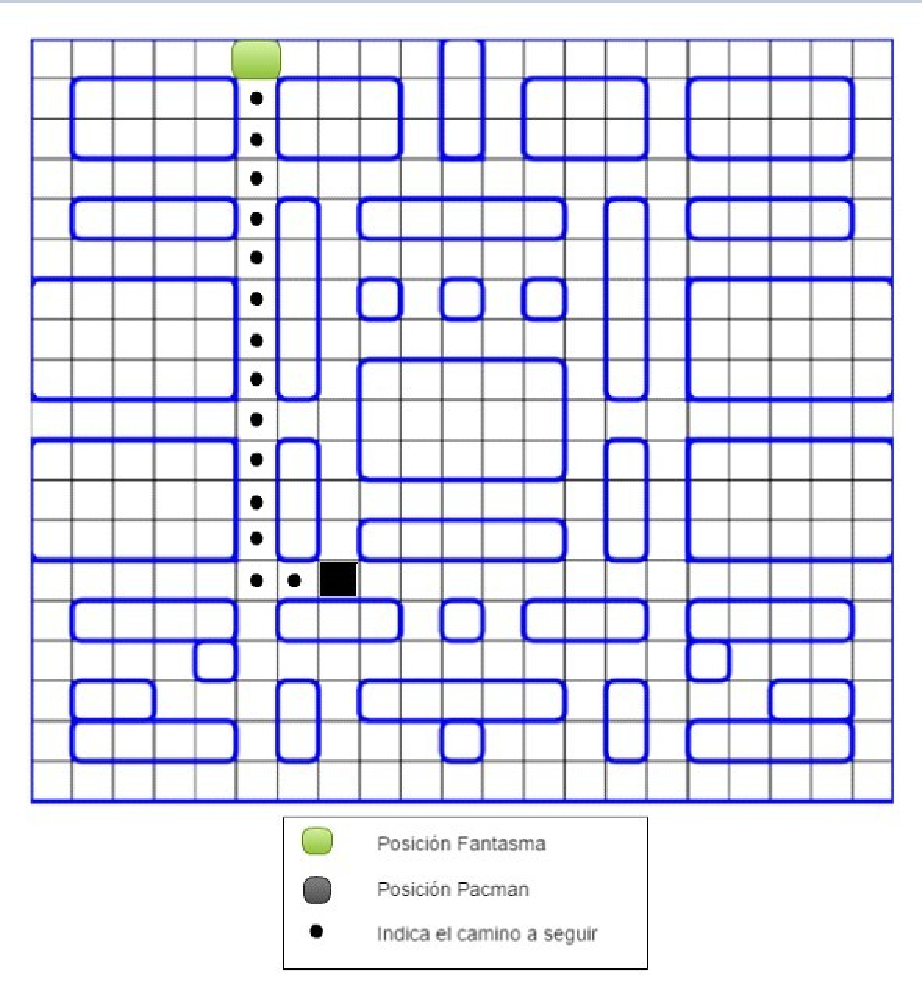
\includegraphics[width=0.5\linewidth, height=8cm]{Figures/InteligenciaArtificial}
	\decoRule
	\caption[InteligenciaArtificial Fantasmas]{InteligenciaArtificial Fantasmas.}
\label{fig:InteligenciaArtificial}
\end{center}
\end{figure}

\subsection{Esquema}
Se presenta un esquema de los puntos más importantes que nos podemos encontrarnos cuando se
ejecute el código. En cada momento se evalúa el comportamiento de Pacman ya actualizar sus
características depende de los elementos del entorno. \ref{fig:esquemaP1}
\begin{figure}[h]
\centering
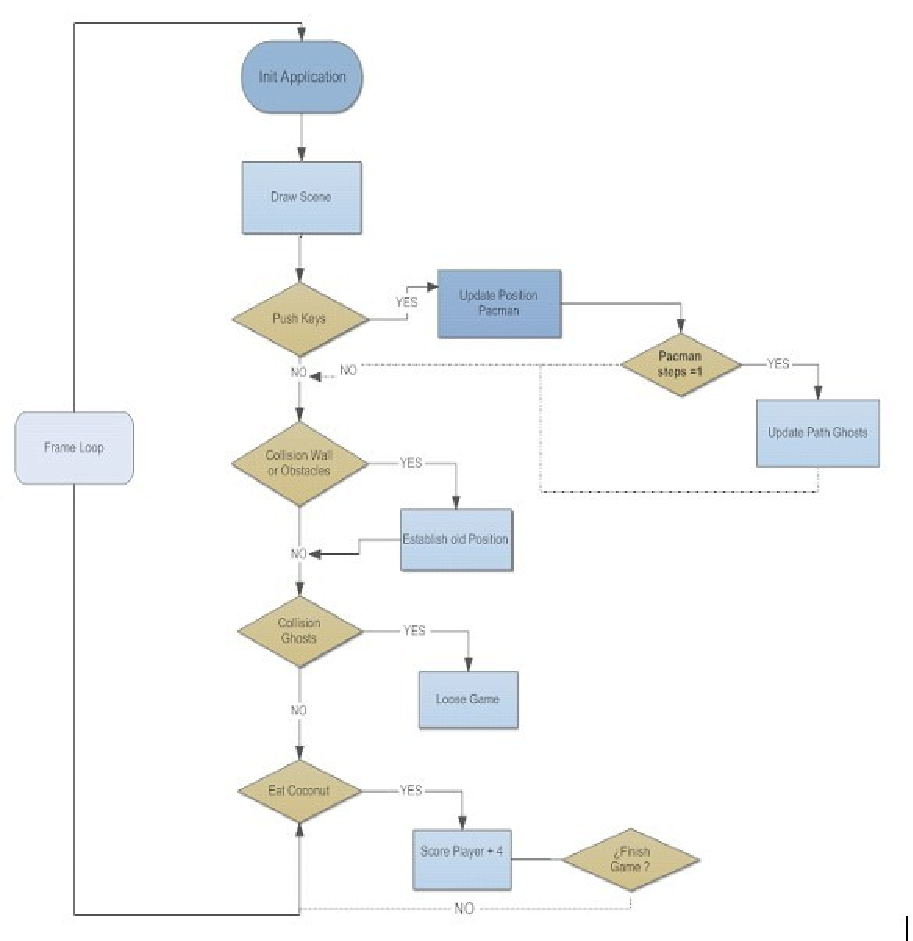
\includegraphics[width=0.8\linewidth]{Figures/esquemaP1}
\decoRule
\caption[An Electron]{An electron (artist's impression).}
\label{fig:esquemaP1}
\end{figure}
\subsection{Desarrollo}
Como se ha dicho a lo largo de este desarrollo la lógica del juego recae sobre JavaScript. Por esto se
han creado tres tipos de objetos (GameArea, Pacman, Ghost) con el objetivo de hacer más compacto
el código y menos repetitivo ya que hay muchas funciones que tienden a repetirse.
A continuación, explicaremos cada objeto la función que tienen en el juego
\subsection{GameArea}
Se define el área donde se reproduce la acción del juego. Las principales acciones que tiene que
realizar son las siguientes:
\begin{enumerate}
\item \textbf{contexto juego} \\ Es el punto de partida para utilizar ‘canvas' y su posterior manipulando con JavaScript. ++++ falta los contenedores de codigo +++++
\item \textbf{renderizar} \\ Esta función se encargada de renderizar el 'canvas' en el intervalo de tiempo definido, visualizando
el contenido que ha cambiado. Utilizamos un evento time de JavaScript, al que se le pasa el nombre
de la función que contiene toda la lógica del dibujo y el intervalo de ejecución \lstset{language=C, breaklines=true, basicstyle=\footnotesize}
\lstset{numbers=left, numberstyle=\tiny, stepnumber=1, numbersep=-2pt}
%linewidth=11cm
\begin{lstlisting}[
frame=single,
commentstyle=\color{CadetBlue},
captionpos=b,
caption=Incluir elementos multimedia remotos l.]
   SetInterval(UpdateGameArea,100)
\end{lstlisting}
\item \textbf{dibujar elementos básicos} \\ Definimos un conjunto de funciones asociadas al área de juego correspondientes a elementos
estáticos que aparecen en el juego.

\item \textbf{Obstáculos} \\ Definimos un array de obstáculos con las características (posición, ancho, largo) necesarias
para dibujarlos.\lstset{language=C, breaklines=true, basicstyle=\footnotesize}
\lstset{numbers=left, numberstyle=\tiny, stepnumber=1, numbersep=-2pt}
%linewidth=11cm
\begin{lstlisting}[
frame=single,
commentstyle=\color{CadetBlue},
captionpos=b,
caption=Incluir elementos multimedia remotos l.]
 draw_obstacles : function(list){
  for(var i=0;i<list.length;i++){
    var elemento = list[i]; 
    this.context.fillRect(elemento.x*40,elemento.y*40,elemento.width*40,elemento.height*40);
   }
},
\end{lstlisting}
\item \textbf{Cocos} \\ Al igual que los obstáculos generamos un array de cocos con sus características.\lstset{language=, breaklines=true, basicstyle=\footnotesize}
\lstset{numbers=left, numberstyle=\tiny, stepnumber=1, numbersep=-2pt}
%linewidth=11cm
\begin{lstlisting}[
frame=single,
commentstyle=\color{CadetBlue},
captionpos=b,
caption=Incluir elementos multimedia remotos l.]
 draw_doits : function(lista){
  if(lista.length > 0){ 
   for(var i=0;i<lista.length;i++){ 
    var elemento = lista[i]; 
    this.context.fillStyle = 'white'; 
    this.context.beginPath(); 
    this.context.arc((elemento.x*40)+20,(elemento.y*40)+20,elemento.radio,0,(Math.PI/180),true);
    this.context.fill();
   }
 }
},
\end{lstlisting}
\item \textbf{Grid} \\ Esta parte del dibujo es más bien una ayuda que utilizamos durante el desarrollo ya que nos
permite controlar la posición de los elementos de una mejor manera.
\lstset{language=, breaklines=true, basicstyle=\footnotesize}
\lstset{numbers=left, numberstyle=\tiny, stepnumber=1, numbersep=-2pt}
%linewidth=11cm
\begin{lstlisting}[
frame=single,
commentstyle=\color{CadetBlue},
captionpos=b,
caption=Incluir elementos multimedia remotos l.]
 grid : function(){ 
  for(var i=0;i<21;i++){ 
    for(var j=0;j<19;j++){ 
      this.context.strokeStyle="black"; 
      this.context.strokeRect(i*this.value_cuad,j*this.value_cuad, this.value_cuad, this.value_cuad); 
     }
   }
} 
\end{lstlisting}
\item \textbf{Información partida} \\ Tenemos que mostrar al usuario información relacionada con datos de la partida, por esto se
ha defino una función que se encarga contar la puntuación que el usuario tiene en cada
movimiento y otra que nos indica de cuántas vidas disponemos por partida, por defecto
todas las partidas tienen una.

\item Cronómetro \\ Establecemos un contador de tiempo para que el usuario sepa cuanto tiempo ha empleado
en terminar la partida.
\lstset{language=, breaklines=true, basicstyle=\footnotesize}
          \lstset{numbers=left, numberstyle=\tiny, stepnumber=1, numbersep=-2pt}
          %linewidth=11cm
          \begin{lstlisting}[
          frame=single,
          commentstyle=\color{CadetBlue},
          captionpos=b,
          caption=Incluir elementos multimedia remotos l.]
            function draw_time(){ 
              if(start_crono == true){ 
                seconds += 1; 
                  if(seconds > 60){ 
                     min += 1; seconds = 0; 
                   } 
                   if(min > 60){ 
                      horas += 1; min = 0; 
                   } 
                } 
              GameArea.time = horas+':'+min+':'+seconds; 
              setTimeout(draw_time,1000);
           }
          \end{lstlisting}

%Definimos el siguiente timer ‘setTimeout(draw_time,1000)’ el cual se encarga de contar los segundos que han pasado desde el inicio de la partida.
\end{enumerate}

\subsection{Pac-Man}
Es el protagonista del juego y por ende el usuario interactúa con el moviéndolo por todo el
escenario. En su lógica tenemos que tener en cuenta diversos factores que afectan en su progreso
por el juego que explicaremos a continuación.
\begin{enumerate}
\item \textbf{Actualizar posición} \\ Se vincula el evento 'downKey' al canvas y comprobaremos que la tecla que se ha presionado sea
una de las cuatro fechas para actualizar la posición. Esta actualización consiste en sumar o restar 0.5
unidades a la posición actual de Pacman lo que produce el movimiento en la dirección seleccionada.\\Pero aún nos queda comprobar el número de pasos que ha dado ya que tenemos que actualizar su
posición en nuestro mapa de juego. Para controlar esta actualización dispone de una variable
llamada 'pasos':
 * Si es mayor a 1 significa que se ha movido una casilla completa y activa un flag que sirve
como aviso para que los fantasmas actualicen su camino hacia él.
 *Si es menos a 1 solo se suma 0.5 que es la cantidad de espacio que se ha movido Pacman 
 
\item \textbf{Detectar colisiones} \\ Tenemos que comprobar que Pacman se desplace a una posición valida por ello dispone de la
función ‘hitObject ()’ la cual aplica el método de detección de colisiones explicado anteriormente
entre él y cualquier objeto que necesitemos comprobar (obstáculos y fantasmas)

\item \textbf{ Dibujar} \\ Nos queda definir su función de dibujado en la cual carga una imagen y aplicamos la posibilidad de
%cortar una sección de la imagen correspondiente a Pacman. Se utiliza la variable ‘state_draw’ para
intercambiar entre dos imágenes para crear animación.
\end{enumerate}

\subsection{Fantasmas}
Son los enemigos de Pacman y lo perseguirán por todo el escenario hasta ser capturado. Son en total
tres fantasmas con modos de persecución que varían un poco entre unos y otro puede. que
encontraremos a lo largo del escenario y que tienen como objetivo eliminar al jugador para que
pierda la partida.
El objeto Fantasma está diseñado con las siguientes funcionalidades:
\begin{enumerate}
\item \textbf{Actualizar posición} \\Para actualizar la posición de cada fantasma tenemos una variable que cuenta los pasos que han
dado, cuando este variable es mayor a uno actualizamos la posición de ’x’ e ‘y’ con el primer valor de
la lista de nodos de los que dispone el fantasma.
Escogemos el primer valor debido a que en cada actualización eliminamos un nodo por lo que
siempre en la primera posición estará la siguiente posición.
\item \textbf{Dibujar el fantasma }\\Para dibujar los fantasmas lo hacemos igual que Pacman, pero al tener diferentes fantasmas que
corresponden diferentes valores de nuestra imagen de carga definimos su nombre cuando lo
creamos para que en la función de dibujado sepamos con que parte de la imagen principal está
asociado
\item \textbf{Actualizar objetivo}\\Como mencione en la actualización de posición de Pacman se activaba un flag. Este flag permite que
esta función se active.
Hay que tener en cuenta que cada fantasma es diferente por lo que su forma de obtener los puntos
hacia Pacman lo será igual, a continuación, se explica cada uno.
\begin{itemize}
\item  Blinky: haciendo referencia a la historia del juego, el comportamiento del fantasma es seguir
a Pacman en la misma dirección, entonces el punto de inicio es la posición actual del
fantasma y el punto final es la nueva posición de Pacman.
\item Speedy: al igual que Blinky su comportamiento es seguir a Pacman, pero tiene en cuenta la
dirección en la que Pacman se mueve. En este caso el cálculo se realiza como punto de
partida la posición de Speedy y se consulta la dirección de Pacman y le sumamos/ restamos
4 posiciones según corresponda para obtener el punto final.
\item Clyde : tiene dos tipos de comportamientos que dependen de la distancia entre él y Pacman
, si dicha distancia es mayor a ocho sigue en modo persecución en caso contrario deja de
seguirlo y se aleja de él tomando como objetivo nuevo una de las esquinas.\end{itemize}
\end{enumerate}
	
% -------------------------------------------------------------------------------------------
% Practica PACMAN -- ONLINE
%-------------------------------------------------------------------------------------------
\section{Game multi-player}
% -------------------------------------------------------------------------------------------
% Practica Django
%-------------------------------------------------------------------------------------------
\section{Aplicacion Web}
Se pretende dar a conocer los distintos elementos que son necesesarios en la creacion de una aplicación Web y como estos elementos se conectan entre si.\\El framework seleccionado es Django por su interfaz sencillo en la creacion del contenido  a traves de la pagina de adminsitracion y porque se desarrola en python.
La aplicacion tiene como tema festivales y cantantes  en la que se pretente abarcar los siguientes puntos como requisitos en el desarrollo
\subsection{Requisitos}
Presentamos a continuacion los requisitos de la practica con el objetivo de tener una vision amplia del framework con el que vamos a trabajar.
\begin{enumerate}
\item Varias url's,model's,view's
\item Utilizar contenido multimedia
\item Autocompletado con Ajax
\item BBDD MySQL
\item Mapas (Google Map)
\item Gestion de Usuarios
\item Carrito de la compra
\item Formularios
\end{enumerate}
\subsection{Tecnicas Implementadas}
\subsubsection{Model}
Son clases definidas en el archivo 'models.py' que corresponden a tablas generadas en la BBDD definida en la aplicacion web. 
\\La creacion de los 'models' se realizan a traves del objeto Model del que dispone Django. Este objeto permite establecer el tipo de dato correspondiente a  cada campo del modelo dentro de las caracteristicas tenemos que destacar  tres metodos que permiten relacionar un campo de un modelo con otro modelo distinto.
\begin{itemize}
\item ForeignKey :  establece una relacion una a una
\item OnetoOne : relacion uno a uno
\item ManyToManyField: establece la relacion una a muchos.
\end{itemize}
En la practica se utilizan fundamental los dos primeros tipos para relacionar las modelos\footnote{Anexo 3 Modelos}entre si.
\subsubsection{URL's}
Definimos una serie de direcciones(url's) a traves de las cuales se redirecciona al cliente a nueva pagina. La url se define como una dupla en la que el primer elemento es el path de la url  y el segundo es la vista que se ejecuta para obtener el contenido de la nueva pagina.
\\Hay que mencionar que a traves del path podemos pasar parametros \footnote{http://boook.Django}que posteriormente lo utilizara la vista correspondiente .a su vez seran utilizados en la vista 
\begin{lstlisting}[
frame=single,
commentstyle=\color{CadetBlue},
captionpos=b,
caption=Incluir elementos multimedia remotos l.]
 #direccion con parametro adicional
 url(r'^artista/(?P<singer>\w{1,50})/$', views.CantanteSelect),
 #direccion sin parametro
 url(r'^videos/$', views.IndexView),
\end{lstlisting}
\subsubsection{View}
Conjunto de funciones que se encuentran dentro del archivo 'views.py' que se encargan de tratar las peticiones realizadas por el cliente.En el tratamiento de las peticiones se realizan consulta contra la BBDD para obtener la informacion requerida.
\\La consulta dentro de la BBDD se realiza a traves del interfaz del que dispone Django lo que facilita las consultas ya que disvincula el tipo de BBDD con la que se trabaja.
\subsubsection{Template}
Este nombre reciben los documento html en los que se vuelca la informacion obtenida en una consulta para ser presentada al usuario.Para realizar esta tarea es necesario que dentro del  documento html se utilize el lenguaje de plantilla\footnote{http://boook.Django} que nos permiten acceder a la informacion y presentarla segun nuestras necesidades.
\\Una de las caracteristicas destacables es la herencia entre plantillas ,es decir, se define en una plantilla base los elementos que no son comunes y se encierran entra las sentencias 'block nameBlock'  y 'endBlock',mientras que las plantillas hijas comienzan con la siguiente sentencia 'extends AppBase.html' y colocar el nuevo contenido entre las sencias que se han establecen en la plantilla padre.

\subsubsection{Cookie}
Las cookies son información que se almacena en el navegador de forma persistente, es decir, que no desaparece cuando el usuario navega a través de diferentes urls. Además, las cookies son enviadas al servidor cuando el usuario hace una petición, de modo que el servidor puede conocer esa información y actuar en consecuencia.
\\Para ello disponemos del metodo  'setCookie' que nos permite guardar informacion del usuario dentro de la cookie. 
\\codec setCookie
\\Otro metodo es 'getCookie' que permite realizar consultas sobre la informacion de un determinado usuario dentro de la cookie.
\\codec set cookies

\subsubsection{Ajax}
Con AJAX no es necesario recargar toda la página web, como ocurre cuando pinchamos en un enlace o cuando pulsamos el botón submit de un formulario. Es posible realizar una conexión a un servidor desde dentro de una página web usando un programa Javascript. Dicho servidor enviará una respuesta; esta respuesta se almacenará en una variable del programa Javascript y, una vez almacenada en la variable, podremos hacer con ella lo que deseemos.
\\Existen varias formas formas de desarrollar esto en nuestro caso lo haremos a traves de Jquery que dispone de un metodo 'ajax.()' 
\\codec ajax
\subsubsection{Google Maps}
Se ha desarrollo un paquete JS por parte de Google Maps que permite incluir dentro de una web mapas y trabajar con ellos.Para utilizarlo necesitamos generar un clave la cual se obtiene a traves de la pagina oficial de google \footnote{http://googlemaps.com} y se incluye dentro del documento html mediante el script del paquete.
\\ codec js 
\\ Para visualizar el mapa es necesario definir en el cuerpo del documento la etiqueta '<map>' ya que es donde se vuelca la informacio del mapa solicitado. No solo permite obtener un mapa especifico sino añadir marcadores, dibujar sobre él entre otras tareas a traves de los pequeños paquetes de los que dispone el paquete.La comunicacion del paquete para obtene la informacion se realiza a traves de Ajax donde los datos viajan en formato JSON transparente al desarrollador.
\\ codec example \\
\subsection{Implementación}
\subsubsection{Conexion BBDD}
Utilizaremos como BBDD MySQL , para ello es necesario instalar 3 controladores que permiten establecer la conexion entre Django y BBDD .
\\Una vez, se han instalado los componentes necesarios para la conexion tenemos que incluir en el fichero 'setting.py',  los datos de la BBDD para que Django se conecte.
\begin{lstlisting}[
frame=single,
commentstyle=\color{CadetBlue},
captionpos=b,
caption=Incluir elementos multimedia remotos l.]
 DATABASES = {
    'default': {
        'ENGINE': 'django.db.backends.mysql',
        'NAME': 'prueba',
        'USER':'root',
        'PASSWORD':'*******',
        'HOST':'',
        'PORT':'',
    }
 }
\end{lstlisting}
Con esto tenemos la conexion establecida, el siguiente paso es rellenar la BBDD por lo que lo realizamos a traves de fichero models.py que se encuentra dentro del proyecto.
\subsubsection{ToolBar}
\textbf{Galeria}
\\El usuario pulsa el enlace 'Galeria' que provoca la redireccione a la url definida en el archivo 'urls.py' correspondiente a imagenes. A su vez provoca la ejecucion de la funcion 'IndexImagenes' que realiza una consulta a BBDD sobre las imaganes disponibles.
\begin{lstlisting}[
frame=single,
commentstyle=\color{CadetBlue},
captionpos=b,
caption=Incluir elementos multimedia remotos l.]
 #urls.py
 url(r'^imagenes/$', views.IndexImagenes),

 #models.py
 def IndexImagenes(request):
  list_img=Imagenes.objects.all()
  return render(request,'imgAll.html',{'list_img':list_img})
\end{lstlisting}
El resultado de la consulta se renderiza en el archivo 'imgAll.html'. A cada  imagen vinculamos una funcion la cual al pulsarla se coloca en primer plano a traves de una ventana emergente.
\\Estes efecto lo realizamos a traves del evento 'Modal' del que dispone Boostrap, ya que esto lo definimos el archivo html \footnote{Anexo 3 Templates}.
\begin{lstlisting}[
frame=single,
commentstyle=\color{CadetBlue},
captionpos=b,
caption=Incluir elementos multimedia remotos l.]
 function nextModal(file){
  var path = '/media/'+file;
  $('#view').attr('src', path);
 }
\end{lstlisting}
\textbf{Videos}
\\El usuario pulsa el enlace 'Videos' que provoca la redireccione a la url definida en el archivo 'urls.py' correspondiente a videos. A su vez provoca la ejecucion de la funcion 'IndexView' que realiza una consulta a BBDD sobre los videos disponibles.
\lstset{language=, breaklines=true, basicstyle=\footnotesize}
\begin{lstlisting}[
frame=single,
commentstyle=\color{CadetBlue},
captionpos=b,
caption=Incluir elementos multimedia remotos l.]
 #urls.py
 url(r'^videos/$', views.IndexView),
 
 #models.py
 def IndexView(request):
   list_video=Videos.objects.all()
   return render(request,'fullVideo.html',{'list_video':list_video})
\end{lstlisting}
El resultado de la consulta se renderiza en el archivo 'fullVideo.html'. Al disponer de dos tipos de archivos cuando el usuario seleccione un video se activa la funcion 'play repro' la cual evalua que tipo de archivo es y lo presenta en la correspondiente etiqueta. 
\begin{lstlisting}[
frame=single,
commentstyle=\color{CadetBlue},
captionpos=b,
caption=Incluir elementos multimedia remotos l.]
 function play_repro(file,tipo){
  if(tipo == 'iframe'){
   $('iframe').attr("src",file);
   $("video").hide();
   $("iframe").show();
  }else{
  var path ='/media/'+file;
  $('video').attr("src",path);
  $("iframe").hide();
  $("video").show();
  }
 }
\end{lstlisting}
\textbf{Artistas}
\\El usuario pulsa el enlace 'Artitas' que genera un desplegable con los nombres de los artistas disponibles. Tras la seleccion del artista se redirecciona a la url definida en el archivo 'urls.py' correspondiente a artistas.
\\A su vez provoca la ejecucion de la funcion 'CantanteSelect' que recibe como parametro adicional el nombre del artitas que se utiliza en la consulta a BBDD.
\begin{lstlisting}[
frame=single,
commentstyle=\color{CadetBlue},
captionpos=b,
caption=Incluir elementos multimedia remotos l.]
 #urls.py
 url(r'^artista/(?P<singer>\w{1,50})/$', views.CantanteSelect),
 
 #models.py
 def CantanteSelect(request,singer):
   cantante = Artista.objects.get(name=singer)
   return render(request,'Artista.html',{'cantante':cantante})
\end{lstlisting}
El resultado de la consulta se renderiza en el archivo 'Artista.html'.En la seccion de discos de la pagina se vincula a cada disco la funcion 'loadcancion' que se encarga de generar un lista de reproduccion con los canciones asociadas a dicho disco. Esta lista se representa como una tabla en la cual encontramos el nombre de las canciones y al pinchar en una de ellas reproducimos el contenido.
\begin{lstlisting}[
frame=single,
commentstyle=\color{CadetBlue},
captionpos=b,
caption=Incluir elementos multimedia remotos l.]
 function loadcancion(file){
  var path='/media/'+file;
  $('#repro').attr('src',path);
  var tag = document.getElementById('repro');
  tag.oncanplaythrough  = function() {
    tag.play();
    $('#durationRepro').text(tag.duration);
    $('#stateRepro').text('reproduciendo');
    tag.onended = function(){
     $('#stateRepro').text('');
     };
    };
 }
\end{lstlisting}
\textbf{Festivales}
\\El usuario pulsa el enlace 'Festivales' que genera un desplegable con los nombres de los festivales disponibles. Tras la seleccion del festival se redirecciona a la url definida en el archivo 'urls.py' correspondiente a artistas.
\\A su vez provoca la ejecucion de la funcion 'EventSelect' que recibe como parametro adicional el nombre del festival que se utiliza en la consulta a BBDD.
\lstset{language=, breaklines=true, basicstyle=\footnotesize}
\begin{lstlisting}[
frame=single,
commentstyle=\color{CadetBlue},
captionpos=b,
caption=Incluir elementos multimedia remotos l.]
 #urls.py
 url(r'^eventos/(?P<evento>\w{1,50})/$',  views.EventSelect),
 
 #models.py
def EventSelect(request,evento):
 event = Evento.objects.filter(name__startswith=evento)
 context = {'event':event}
 return render(request,'IndexEvent.html',context)
\end{lstlisting}
El resultado de la consulta se renderiza en el archivo 'IndexEvent.html'.Se añade funcionalidad dentro de la pagina para obtener un mapa cuando se pulse el boton'Ver Mapa' el cual ejecuta la funcion 'initMap(latitud,longitud) '.
La funcion realiza una instancia del mapa con las coordenadas que recibe ademas creemos un marcador el cual al ser pinchado abre una ventana emergente situado de las coordenadas anteriores.
\begin{lstlisting}[
frame=single,
commentstyle=\color{CadetBlue},
captionpos=b,
caption=Incluir elementos multimedia remotos l.]
 function initMap(latitud,longitud) {
  var place = {lat:parseFloat(latitud),lng:parseFloat(longitud)};
  
  //Creamos la instacia del mapa
  var map = new google.maps.Map(document.getElementById('mapholder'), {
    center: place,
    scrollwheel: false,
    zoom: 10
  });
  
  //Creamos una marcador para el mapa
  var marker = new google.maps.Marker({
   position: place,
   map: map,
   title: 'Concierto',
   draggable: true,
   animation: google.maps.Animation.DROP,
  });
  
  var contentString ='Localizacion del concierto';
  // Creamos una venta de informacion
  var infowindow = new google.maps.InfoWindow({
    content: contentString
  });
  
  // Anadimos un evento al marker
  marker.addListener('click', function() {
     infowindow.open(map, marker);
   });
 }
 \end{lstlisting}
\subsubsection{Gestión de Usuarios}
Para poder trabajar con usuarios definimos una serie de funcionalidades dentro de la web tales como Registrer,Login,Perfil del Usuario y Logout.
\\
\\\textbf{\textit{Register}}
\\Permite guarda nuevos usuarios dentro de la BBDD . El usuario pincha en el enlace 'Register' eel cual genera un para ello el usuario necesita rellenar la informacion de un formulario que sera validado en el servidor.necesitan realizar este proceso para formar parte del grupo de usuarios, disponer de un perfil y un registro de la compras realizadas.
\\El usuario pulsa el enlace 'Register' que provoca la redireccion a la url definida en el archivo 'urls.py' correspondiente al registro de usuarios. Esto provoca la ejecucion de la funcion 'indexRegister' la cual define su comportamiento dependiendo del tipo de metodo que presenta la solicitud. Si es 'GET' la funcion genera un formulario vacio el cual sera entregado al cliente mientras si es'POST' significa que el usuario ha rellenado el formulario en este caso obtenemos la informacion del cuerpo del mensaje y la validamos.
Con esta informacion generamos una  nuevo  usuario con 'User.objects.create user()'que realiza una consulta a BBDD sobre las imaganes disponibles.
\\A su vez provoca la ejecucion de la funcion 'EventSelect' que recibe como parametro adicional el nombre del festival que se utiliza en la consulta a BBDD.
\\Cuano el usuario pincha en el icono de register realiza la peticion al servidor el cual se encarga de gestionarla a traves de la funcion ' '. La funcion se encarga de evaluar el metodo de la peticion ya que si es 'GET'  se envia el formulario vacio mientras que si es 'POST'  se trata del  formulario relleno por lo que es necesario obtener la informacion del cuerpo del mensaje para ser validada.
\lstset{language=, breaklines=true, basicstyle=\footnotesize}
\begin{lstlisting}[
frame=single,
commentstyle=\color{CadetBlue},
captionpos=b,
caption=Incluir elementos multimedia remotos l.]
  #urls.py
 url(r'^register/$',  views.indexRegister),

 #models.py
 def indexRegister(request):
  if request.method == 'POST':
   formRegister = Register(request.POST)
    if formRegister.is_valid():
     user = formRegister.cleaned_data['nick']
     nombre = formRegister.cleaned_data['nombre']
     apellido = formRegister.cleaned_data['apellido']
     password = formRegister.cleaned_data['pasword']
     email = formRegister.cleaned_data['email']
     sex = formRegister.cleaned_data['sexo']
     u=User.objects.create_user(username=user,email=email,password=password,first_name=nombre,last_name=apellido)
     #guardamos el usuario y pasamos a crear el perfil
     perfil = UserProfile(user=u,sexo=sex)
     perfil.save();
     return HttpResponseRedirect('/recursos/login')
   else:
     error = 'La informacion no es valida'
  return render(request,'new_user.html',{'form':Register()})
\end{lstlisting}
Si la informacion es valida generamos un nueva entrada enla tabla User a la vez que generamos un perfil con la misma informacion en la tabla PerfilUser, en caso contrario se informa al usuario que los datos enviados no son correctos.
\\ codect validaciones 
\\
\\\textbf{\textit{Login}}
\\Se permite a los usuarios entrar a la web para consultar su perfil o modificarlo ya que esta funcionalidad solo esta diponible para los usuarios existentes den la BBDD. 
\\El usuario accede a traves del enlace 'login' que sera redirigido a la url definida en el archivo 'urls.py' provocando la ejecucion de la funcion 'indexLogin'. La funcion evalua el metodo que posee la peticion en caso de ser el metodo 'GET' entrega el formulario vacio para que el usuario lo rellene , en caso de ser 'POST' significa que el usuario envia el formulario relleno por lo que la funcion tiene que obtener dicha informacion.
\\Con la informacion creamos una instancia del formulario para poder realizar la validacion de los campos con el metodo 'is valid()' en caso de ser valido obtenemos la informacion y antes de utilizar el metodo 'login' realizmos una autenticacion mediante los metodos  de los que dipone Django.
\\Finalmente, antes de devolver la informacion al usuario se asocia una cookie a la respues con el objetivo de guardar informacion del usuario. 
\begin{lstlisting}[
frame=single,
commentstyle=\color{CadetBlue},
captionpos=b,
caption=Incluir elementos multimedia remotos l.]
def indexLogin(request):
 if request.method == 'POST':
  FormLogins = FormLogin(request.POST)
   if FormLogins.is_valid():
    user = FormLogins.cleaned_data['nombre']
	password = FormLogins.cleaned_data['pasword']
	usuario = authenticate(username=user,password=password) 
	if usuario is not None and usuario.is_active:
	  login(request,usuario)
	  if 'name' in request.COOKIES:
	   if request.COOKIES['name'] == user:
	    cookies = HttpResponseRedirect('/recursos/')
		expires = datetime.datetime.strftime(datetime.datetime.utcnow(), "%a, %d-%b-%Y %H:%M:%S GMT")
		cookies.set_cookie(user,'')
		return cookies
	  else:
	    cookies = HttpResponseRedirect('/recursos/')
		cookies.set_cookie(user,'')
		print request.COOKIES
		return cookies
   else:
     mensaje = "Usuario y/o password incorrecto"
 FormLogins = FormLogin()
 context = {'form':FormLogins}
 return render_to_response('login.html',context,context_instance=RequestContext(request))
\end{lstlisting}
\textbf{\textit{Perfil Usuario}}
\\Para poder trabajar con perfiles tenemos que modificar el archivo 'settings.py' en el que se añade la autorizacion para generar perfiles a traves del modelo User de Django ademas de crear el modelo correspondiente.
\lstset{language=, breaklines=true, basicstyle=\footnotesize}
\begin{lstlisting}[
frame=single,
commentstyle=\color{CadetBlue},
captionpos=b,
caption=Incluir elementos multimedia remotos l.]
#settings.py
AUTH_PROFILE_MODULE = "polls.mysiteprofile"
\end{lstlisting}
El usuario a traves del enlace 'Perfil' obtiene un desplegable con las opciones de las que dispone. Una de ellas es la consulta del perfil en la cual  redireccionamos al usuario a la url  definida en 'urls.py'. Esto a su vez provoca la ejecucion de la funcion 'IndexPerfil.html' que realiza una consulta a BBDD con el nombre del usuario dentro del modelo UserProfile.
\lstset{language=, breaklines=true, basicstyle=\footnotesize}
\begin{lstlisting}[
frame=single,
commentstyle=\color{CadetBlue},
captionpos=b,
caption=Incluir elementos multimedia remotos l.]

#view.py
def IndexPerfil(request):
 infoPerfil=UserProfile.objects.get(user=request.user)
 modif = False
 return render(request,'Perfil.html',{'info':infoPerfil,'modif':modif})
\end{lstlisting}
La ultima opcion disponible es modificar el perfil en la cual se redirecciona al usuario a la url correspondiente dentro del archivo 'urls.py'.Esto hace que la funcion 'ModifPerfil' se ejecuta verificando el metodo con el que se realiza la peticion. Si es 'GET' se envia un formulario lleno de la informacion del usuario mientras que si es 'POST' se genera una instancia del formulario con la nueva informacion que el usuario a enviado/modificado  y se guarda la informacion.
\lstset{language=, breaklines=true, basicstyle=\footnotesize}
\begin{lstlisting}[
frame=single,
commentstyle=\color{CadetBlue},
captionpos=b,
caption=Incluir elementos multimedia remotos l.]

#views.py
 def ModifPerfil(request):
  infoPerfil=UserProfile.objects.get(user=request.user)
   if request.method == 'POST':
    #creamos un formulario con los datos
    newPerfil=FormModifPerfil(request.POST,request.FILES)
    #Sacamos el valor del form y update el perfil
    if newPerfil.is_valid():
     infoPerfil.imgPerfil=newPerfil.cleaned_data['imgPerfil']
     infoPerfil.save()
     return HttpResponseRedirect("/recursos/account")	
   form = FormModifPerfil(instance=infoPerfil)
   modif = True
   return render(request,'Perfil.html',{'form':form,'modif':modif})
\end{lstlisting}
\textbf{\textit{Logout}}
\\Si se pulsa logout el usuario realiza una peticion para cerrar la sesion que tiene abierto.
\lstset{language=, breaklines=true, basicstyle=\footnotesize}
\begin{lstlisting}[
frame=single,
commentstyle=\color{CadetBlue},
captionpos=b,
caption=Incluir elementos multimedia remotos l.]
def IndexLogout(request):
	logout(request)
	res = HttpResponseRedirect("/recursos/")
	return res
\end{lstlisting}
\subsubsection{Carrito de la compra}
Se crea un carrito de la compra basado en cookies como metodo para guardar el estado del cliente durante su estancia en la web.El usuario visualiza el contenido al pulsar el icono del carrito que tiene vinculado la funcion 'ViewCar' quien se apoya en la funcion 'getCookie' para obtener la informacion asociada al usuario.
\lstset{language=, breaklines=true, basicstyle=\footnotesize}
\begin{lstlisting}[
frame=single,
commentstyle=\color{CadetBlue},
captionpos=b,
caption=Incluir elementos multimedia remotos l.]
function View_Car(existe){
 $("tr").remove('#colum');
 if(existe != null){
  var old_item = JSON.parse(existe);
  var obj = JSON.parse(old_item);
  for(var i=0;i < obj.length;i++){
   var compra = obj[i];
   $('#vCookie').append('<tr id=colum >
    <td><img width=60 src=/media/'+compra.imagen+'></td>
    <td>'+compra.nproduct+'</td>
    <td>'+compra.cantidad+'</td> <td>'+compra.total</td>
    <td><button id=delete_'+compra.nproduct+' >eliminar</a></td></tr>');
    $('#delete_'+compra.nproduct).click(function(){
          deleteCookie(String(usuario),String(compra.nproduct),String(compra.tipo))});
    }
  }else{
   $('#elementos').append('
     <li><strong>El carrito esta:'+p+'</strong></li>');
    }
 }
\end{lstlisting}    
El usuario al intentar comprar una entrada la añade al carrito esta accion llama a la funcion 'Añadir' que recibe como parametro la informacion del producto y el nombre del usuario. Con el nombre buscamos la informacion previa existente en la cookie mediante la funcion 'getCookie', tras  obtener la informacion evaluamos si hay contenido previo en cuyo caso se añade el nuevo producto a los anteriores en caso contrario el producto sera el primero  y  guardamos  el  contenido con la funcion 'saveCookie'.
\begin{lstlisting}[
frame=single,
commentstyle=\color{CadetBlue},
captionpos=b,
caption=Incluir elementos multimedia remotos l.]
function Anadir(file,names,user,typeTicket,precio,linkTicket){
var numTickets = $('#'+linkTicket).val();
var comprar={'imagen':file,'nproduct':names,'tipo':typeTicket,'cantidad':numTickets,'total':parseInt(precio)*numTickets};     
///buscamos si existe el usuaario con el contenido
var existe = getCookie(user);
console.log(existe);
if(existe != ''){
var old_item = JSON.parse(existe);
var obj = JSON.parse(old_item);
obj.push(comprar);
setCokie(user,JSON.stringify(obj));
}else{
var list =[comprar];
setCokie(user,JSON.stringify(list));
}
}
\end{lstlisting}  
Cuando el usuario realiza la compra del contenido lo hace a traves del boton 'buy'. Con esto realizamos una peticion al servidor en el que la funcion 'IndexBuy' lee la informacion de la cookie que viaja en la peticion a traves del nombre del usuario.
\\Con el nombre del usuario obtenemos el id ddel modelo 'UserProfile' asociado al modelo 'User' ya que con la informacion obtenida de la cookies creamos una nueva entrada la clase 'Buy' y vinculamos este nuevo elemento al perfill del usuario.
\begin{lstlisting}[
frame=single,
commentstyle=\color{CadetBlue},
captionpos=b,
caption=Incluir elementos multimedia remotos l.]
def IndexBuy(request):
	usuario = str(request.user)
	valueCookie = json.loads(request.COOKIES[usuario])
	idUser = User.objects.get(username=usuario)
	inst_usuario = UserProfile.objects.get(user=idUser.id)
	for elemento in valueCookie:
		#creamos la instncia de la compra
		newCompra = Buy()
		newCompra.typeProducto='evento'
		newCompra.typeTicket=elemento['tipo']
		newCompra.cantidad=elemento['cantidad']
		newCompra.total=elemento['total']
		producto = Evento.objects.get(name=elemento['nproduct'])
		newCompra.save()
		newCompra.nameProduct.add(producto)
		inst_usuario.compra.add(newCompra)
        
	cookie = HttpResponseRedirect("/recursos/")
	expires = datetime.datetime.strftime(datetime.datetime.utcnow()
      + datetime.timedelta(seconds=0), "%a, %d-%b-%Y %H:%M:%S GMT")
	cookie.set_cookie(usuario,request.COOKIES[usuario], expires = expires)
	return cookie
\end{lstlisting}  
Si el usuario desea eliminar un  producto del carrito dispone de un boton el cual se vincula a la funcion 'deleteCookie' que recibe el nombre del usuario y el producto que vamos a eliminar.
\lstset{language=, breaklines=true, basicstyle=\footnotesize}
\begin{lstlisting}[
frame=single,
commentstyle=\color{CadetBlue},
captionpos=b,
caption=Incluir elementos multimedia remotos l.]
function deleteCookie(user,producto,tipoTicket){
//buscamos primero el contenido del usuario
var existe = getCookie(user);
if(existe != null){
var contenido=JSON.parse(existe);
var obj=JSON.parse(contenido);
 for(var i=0;i < obj.length;i++){
 var compra = obj[i];
 if(compra.nproduct == producto && compra.tipo == tipoTicket){
  obj.splice(i,1);
  $('#myModal').modal('hide')
	}	
 }
 /* actualizamos el valor de la cookies tras eliminar el contenido  */	
 setCokie(user,JSON.stringify(obj));
 }
}
\end{lstlisting} 
\subsubsection{Barra de busqueda}
Dentro de la web el usuario dispone de una barra de busqueda con la cual puede realizar una busqueda sobre un determinado elemento que le interese.
\\A la barra se le vincula la funcion 'xx' que se encarga de comprobar la longitud del texto introducido en caso de ser menor a tres no se realiza nada mientras que si es mayor a tres empleamos Ajax para realizar la consulta del contenido al servidor.
\\codec xxxxxxxx
\\ La peticion es atendida por el servidor a traves de la funcion 'xxx' la cual realiza la consulta contra la BBDD del elemento que el usuario a introducido  al terminar la consulta el contenido se renderiza el templete 'xx' el cual genera una lista con el contenido.
\\El contenido es presentado al usuario a traves de la funcion definida en la llamada a Ajax cuando en el proceso no existe ningun fallo.
% -------------------------------------------------------------------------------------------
% Practica Web-RTC
%-------------------------------------------------------------------------------------------
\section{Comunicación muti-Peer}
En esta ultima practica vamos a utilizar la API WebRTC que permite establecer una comunicacion Peer-to-Peer entre navegadores.
Se partira de un ejemplo ya resuelto en el libro [WebRTC] donde la comunicacion se realiza entre dos usuarios y transmiten flujo de audio/video entre ellos. Con el objetivo de entender el entendimiento e ir un paso mas alla se implementa los siguientes elementos.
\subsection{Requisitos}
\begin{itemize}
\item Conexion en malla entre los Peer
\item Envio de audio/video 
\item Envio de ficheros y  caracteres 
\item Creacion de salas 
\end{itemize}
\subsection{Técnicas de implementación}
\subsubsection{GetUserMedia}
Es una herramienta por parte de los navegadores que nos permite acceder a los elementos multimedia de los que dispone el ordenador/móvil/tablet  por lo general estos elementos son el micrófono y la web-Cam.
%linewidth=11cm
\begin{lstlisting}[
frame=single,
commentstyle=\color{CadetBlue},
captionpos=b,
caption=Instancia RTCPeerConnection.]
 var items = {
  audio:true,
  video:true
 }
 navigator.getUserMedia(items,connect_items,error_items);
\end{lstlisting}
\subsubsection{Servidor de Señalización( NodeJS +Socket.IO)}
 Es necesario desarrollar un servidor de señalizacion con el objetivo de encaminar los mensajes entre los distintos peer. Aunque la comunicacion final se realiza Peer-to-Peer al utilizar WebRTC es necesario un intercambio previo de informacion entre los nodos como la descripcion de sesion e informacion de red de cada uno de ellos ,este proceso es conocido como señalizacion.
\\Para la creacion del servidor se utiliza NodeJs ya que tiene una complejidada baja.Lo unico que nos queda es definir es el mecanismos mediante el cual enviamos los mensajes para ello utilizamos Socket.IO el que permite una comunicacion bidireccional  y de baja latencia.
\subsubsection{WebRTC}
Consta de 2 API las cuales se explican a continuacion el modo en el que se aplican en el desarrollo de la practica.
\\
\\\textbf{\textit{RTCPeerConection}}
\\A traves del interfaz de la API  permite a WebRTC la comunicación entre el equipo local y el remoto.
Para ello pone a nuestra disposicion una serie de metodos a traves los cuales permite conectarse a un interlocutor remoto permitiendo mantener,controlar y cerrar la conexion.
Para hacer uso de API es necesario realizar una instancia del mismo .En este punto es necesario pasar como parametro los elementos que utilizara la API para aplicar el protocolo ICE en el que intervienen servidores STUN/TURN. 
\begin{lstlisting}[
frame=single,
commentstyle=\color{CadetBlue},
captionpos=b,
caption=Instancia RTCPeerConnection.]
    /* config Ice FrameWork */
    var pc_config = {
        'iceServer':[{'url':'stun:stun.l.google.com:19302'}]
    };
    /* Creacion RTCPeerConnection */
    var pc = new RTCPeerConnection(pc_config);
\end{lstlisting}
Tras realizar la instanciacion tenemos acceso a sus metodos por lo que se han divido en tres tipos de elementos segun el tipo de metodo.
\\
\\\textbf{Media}
\\Para poder trabajar con el flujo de video disponemos de dos metodos.Para el flujo de video local utilizamos el metodo 'addStream'  con el que vinculamos el video a la conexion.
\begin{lstlisting}[
frame=single,
commentstyle=\color{CadetBlue},
captionpos=b,
caption=Incluir elementos multimedia local.]
pc.addStream(streaming)
\end{lstlisting}
Para el flujo de video remoto perteneciente de otros elementos disponemos del metodo 'onaddStream' con el que se vincula el video remoto a la conexion.
\begin{lstlisting}[
frame=single,
commentstyle=\color{CadetBlue},
captionpos=b,
caption=Incluir elementos multimedia remotos.]
    pc.onaddstream = HandlerRemoteMultimedia
\end{lstlisting}
\textbf{Conectividad} 
\\Presentamos aquellos metodos que permiten establecer/guardar infomacion sobre la sesion que se ha creado.
Disponemos del metodo'createOffert' el cual recibe como parametro la descripcion de la sesion.El nodo quien inicia la conexion hace uso de este metodo y de igual forma guardamos la descripcion de la sesion en la instancia de la API a traves del metodo 'setLocalDescription'.
\begin{lstlisting}[
frame=single,
commentstyle=\color{CadetBlue},
captionpos=b,
caption=Incluir elementos multimedia remotos l.]
  pc.createOffert(HandlerOffert,HandlerError,{});
  /* HandlerOffert */
  function HandlerOffert(sessionDescrip){
   pc.setLocalDescription(sessionDescrip);
   .....................................
  }
\end{lstlisting}
En conjunto al metodo anterior disponemos de 'createAnswer'el cual sirve como contestacion de un nodo al recibir el metodo 'createOffert'.
En este momento obtenemos la informacion de la sesion con el que se crea un objeto de tipo 'RTCSessionDescripcion' con dicha informacion y se guarda en la instancia de 'RTCPeerConnection' mediante el evento 'setRemoteDescripcion'.
Finalmente, utilizamos el metodo 'createAnswer' en el igual que se  realiza con 'createOffert'.
 \begin{lstlisting}[
 frame=single,
 commentstyle=\color{CadetBlue},
 captionpos=b,
 caption=Incluir elementos multimedia remotos l.]
   pc.createanswer(HandlerAnswer,HandlerError,{})
   /* HandlerAnswer */
   function HandlerAnwer(sessionDescrip){
   pc.setLocalDescription(sessionDescrip);
   ....................................
   }
\end{lstlisting}
 \textbf{Información Red} 
\\Como se menciono al principio de este punto dijimos que era necesario pasar como parametro xxxx. Con este parametro obtenemos informacion de la red en la que el nodo se esta ejecutando.En cuanto a la informacion de red que necesitamos conocer es la direccion IP:Puerto del nodo para ello la API utiliza el protocolo ICE.
\\La informacion obtenida es muy importante ya que a traves de ella los nodos pueden establecer conexion sin necesidad utilizar un servidor de por medio.Por ello disponemos del metodo 'icecandidate'  con el que obtemos el par IP:Puerto  a traves del servidor TURN/STUN.
\begin{lstlisting}[
frame=single,
commentstyle=\color{CadetBlue},
captionpos=b,
caption=Incluir elementos multimedia remotos l.]
 pc.onicecandidate = HandlerIceCandidate
 /* HandlerIceCandidate */
 function HandlerOffert(sessionDescrip){
  if(event.candidate){
  var iceCandidate = {
   type:'iceCandidate',
   label:event.candidate.sdpMLineIndex,
   id:event.candidate.sdpMid,
   candidate:event.candidate.candidate
  }
  .........................	
 }
\end{lstlisting}
Cuando un nodo recibe esta informacion de otro nodo es necesario guardarlo por lo que utilizamos el metodo 'addIceCandidate' que se encarga de generar un objeto de este tipo con la informacion recibida.
\begin{lstlisting}[
frame=single,
commentstyle=\color{CadetBlue},
captionpos=b,
caption=Incluir elementos multimedia remotos l.]
   pc.addIcecandidate(new RTCIceCandidate(iceCandidate)) 
\end{lstlisting}
\textbf{\textit{DataChannel}}
\\Se trata de la otra API de la que dispone WebRTC . Su interfaz nos permite crear un canal de comunicacion bidireccional entre un par de nodos.
Permite enviar cualquier tipo de dato por lo que en nuestra aplicacion lo utilizaremos para enviar informacion  del chat y enviar los datos de ficheros. A continuacion se muestra los metodos de los que dispone la API.
\begin{lstlisting}[
frame=single,
commentstyle=\color{CadetBlue},
captionpos=b,
caption=Incluir elementos multimedia remotos l.]
  /*  creacion */
  var sendChannel = pc.createDataChannel('nombre   canal',opciones);
  /*  Handlers */
  sendChannel.onopen = HandlerChannelOpen  /*  el canal esta abierto */
  sendChannel.onclose = HandlerChannelClose /* termina la conexion */
  sendChannel.onmessage = HandlerChannelMssg /* recepcion de mensajes */ 
\end{lstlisting}
\subsection{Esquemas}
En la figura \ref{fig:ComunnicacionWebRTC} un esquema con los elementos necesarios para establecer una comunicacion Peer-to-Peer.
\begin{figure}[!h]
\centering
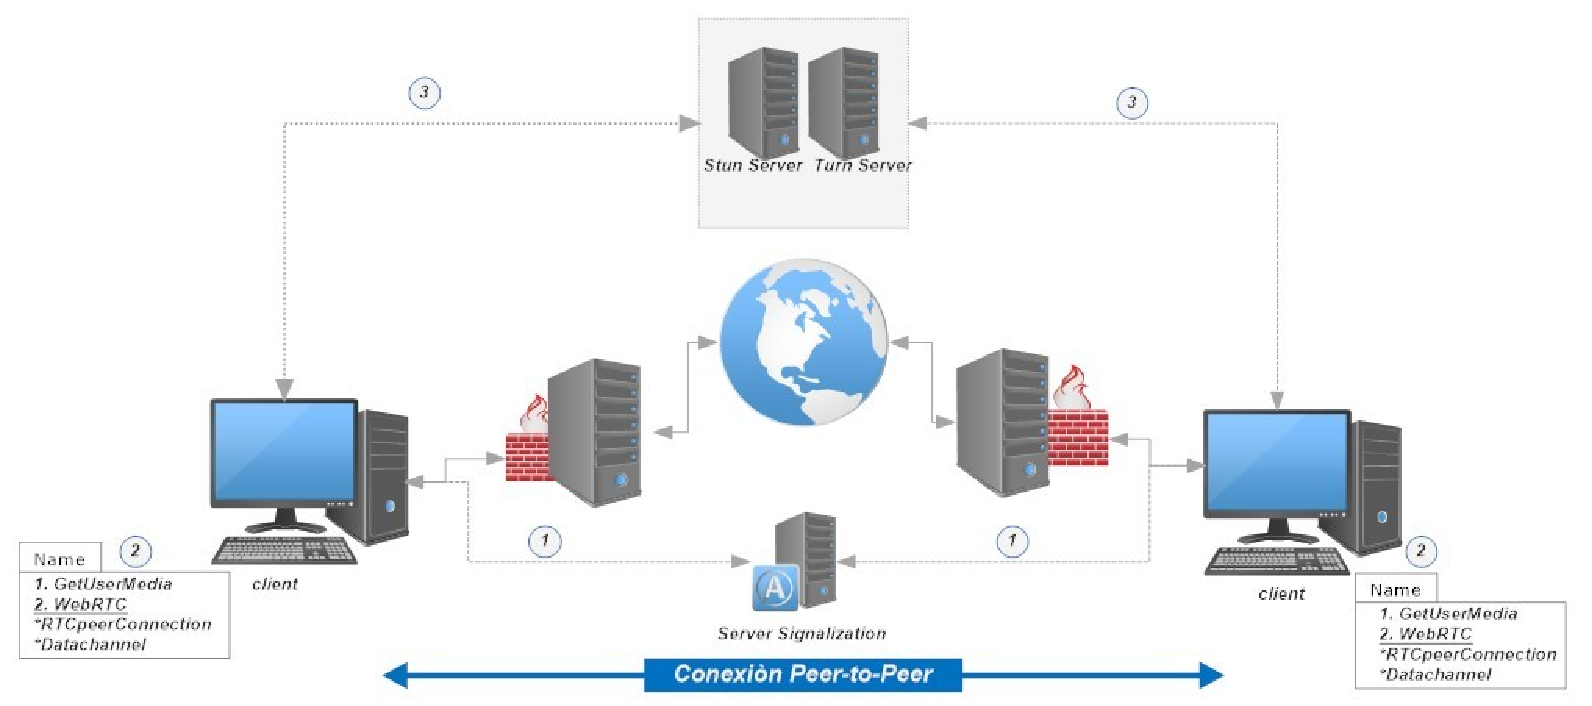
\includegraphics[width=0.6\linewidth]{Figures/ComunnicacionWebRTC}
\decoRule
\caption[An Electron]{ComunnicacionWebRTC (artist's impression).}
\label{fig:ComunnicacionWebRTC}
\end{figure}
\\Tras el proceso de señalizacion la comunicacion entre los nodos es Peer-to-Peer quedando el esquema de comunicacion como en la figura \ref{fig:Conexcion_finish}
\begin{figure}[!h]
\centering
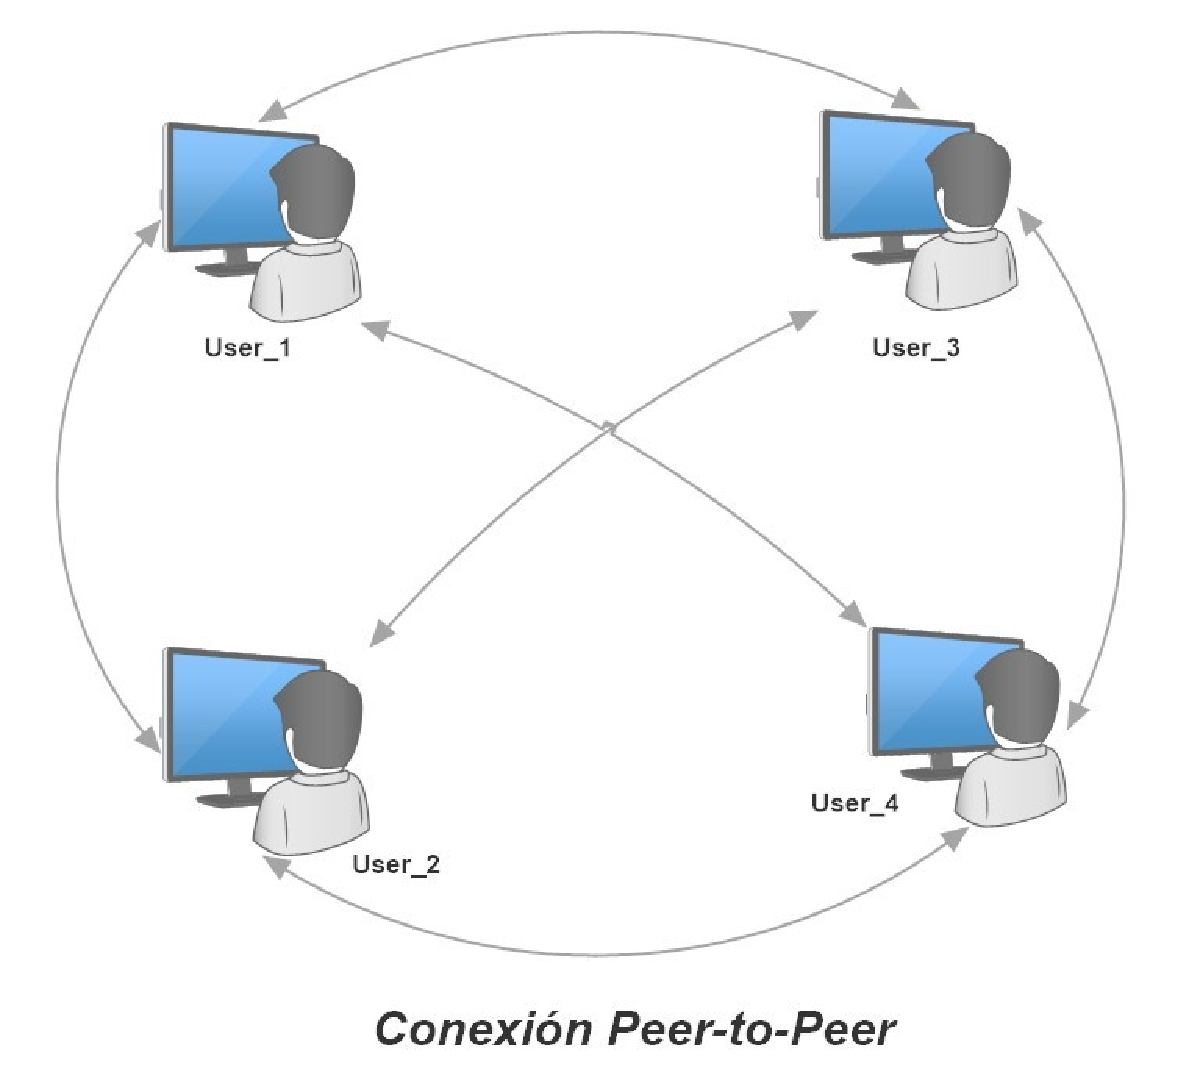
\includegraphics[width=0.6\linewidth]{Figures/Conexcion_finish}
\decoRule
\caption[An Electron]{ComunnicacionWebRTC (artist's impression).}
\label{fig:Conexcion_finish}
\end{figure}
\subsection{Desarrollo}
Una vez explicado el funcionamiento de las tecnologías  que se van a emplear pasamos a describir como se emplean en la realización del desarrollo.
Se va a dividir en dos partes cliente y servidor con el objetivo de explicar de forma adecuada el funcionamiento de cada parte.
\subsubsection{Cliente}
\textbf{Apariencia }
\\El usuario dispone de acceso al toolbar donde encontramos el acceso a la creación de una nueva sala de conexión ,una lista de archivos transmitidos y una lista de de salas existentes, por defecto tiene una sala creada con el nombre 'streaming'.
\\Para seleccionar los elementos multimedia que el usuario quiere intercambiar dispone de dos 'radioButton' de Audio y Video. 
\\El cuerpo de la aplicacion esta dedicado para visualizar el video local e ir añadiendo los videos remotos a medida que se producen  nuevas conexiones.Finalmente el usuario dispone de un chat par
a comunicarse con los usuarios de las salas cuando la conexion se ha establecido.
\begin{figure}[h]
\centering
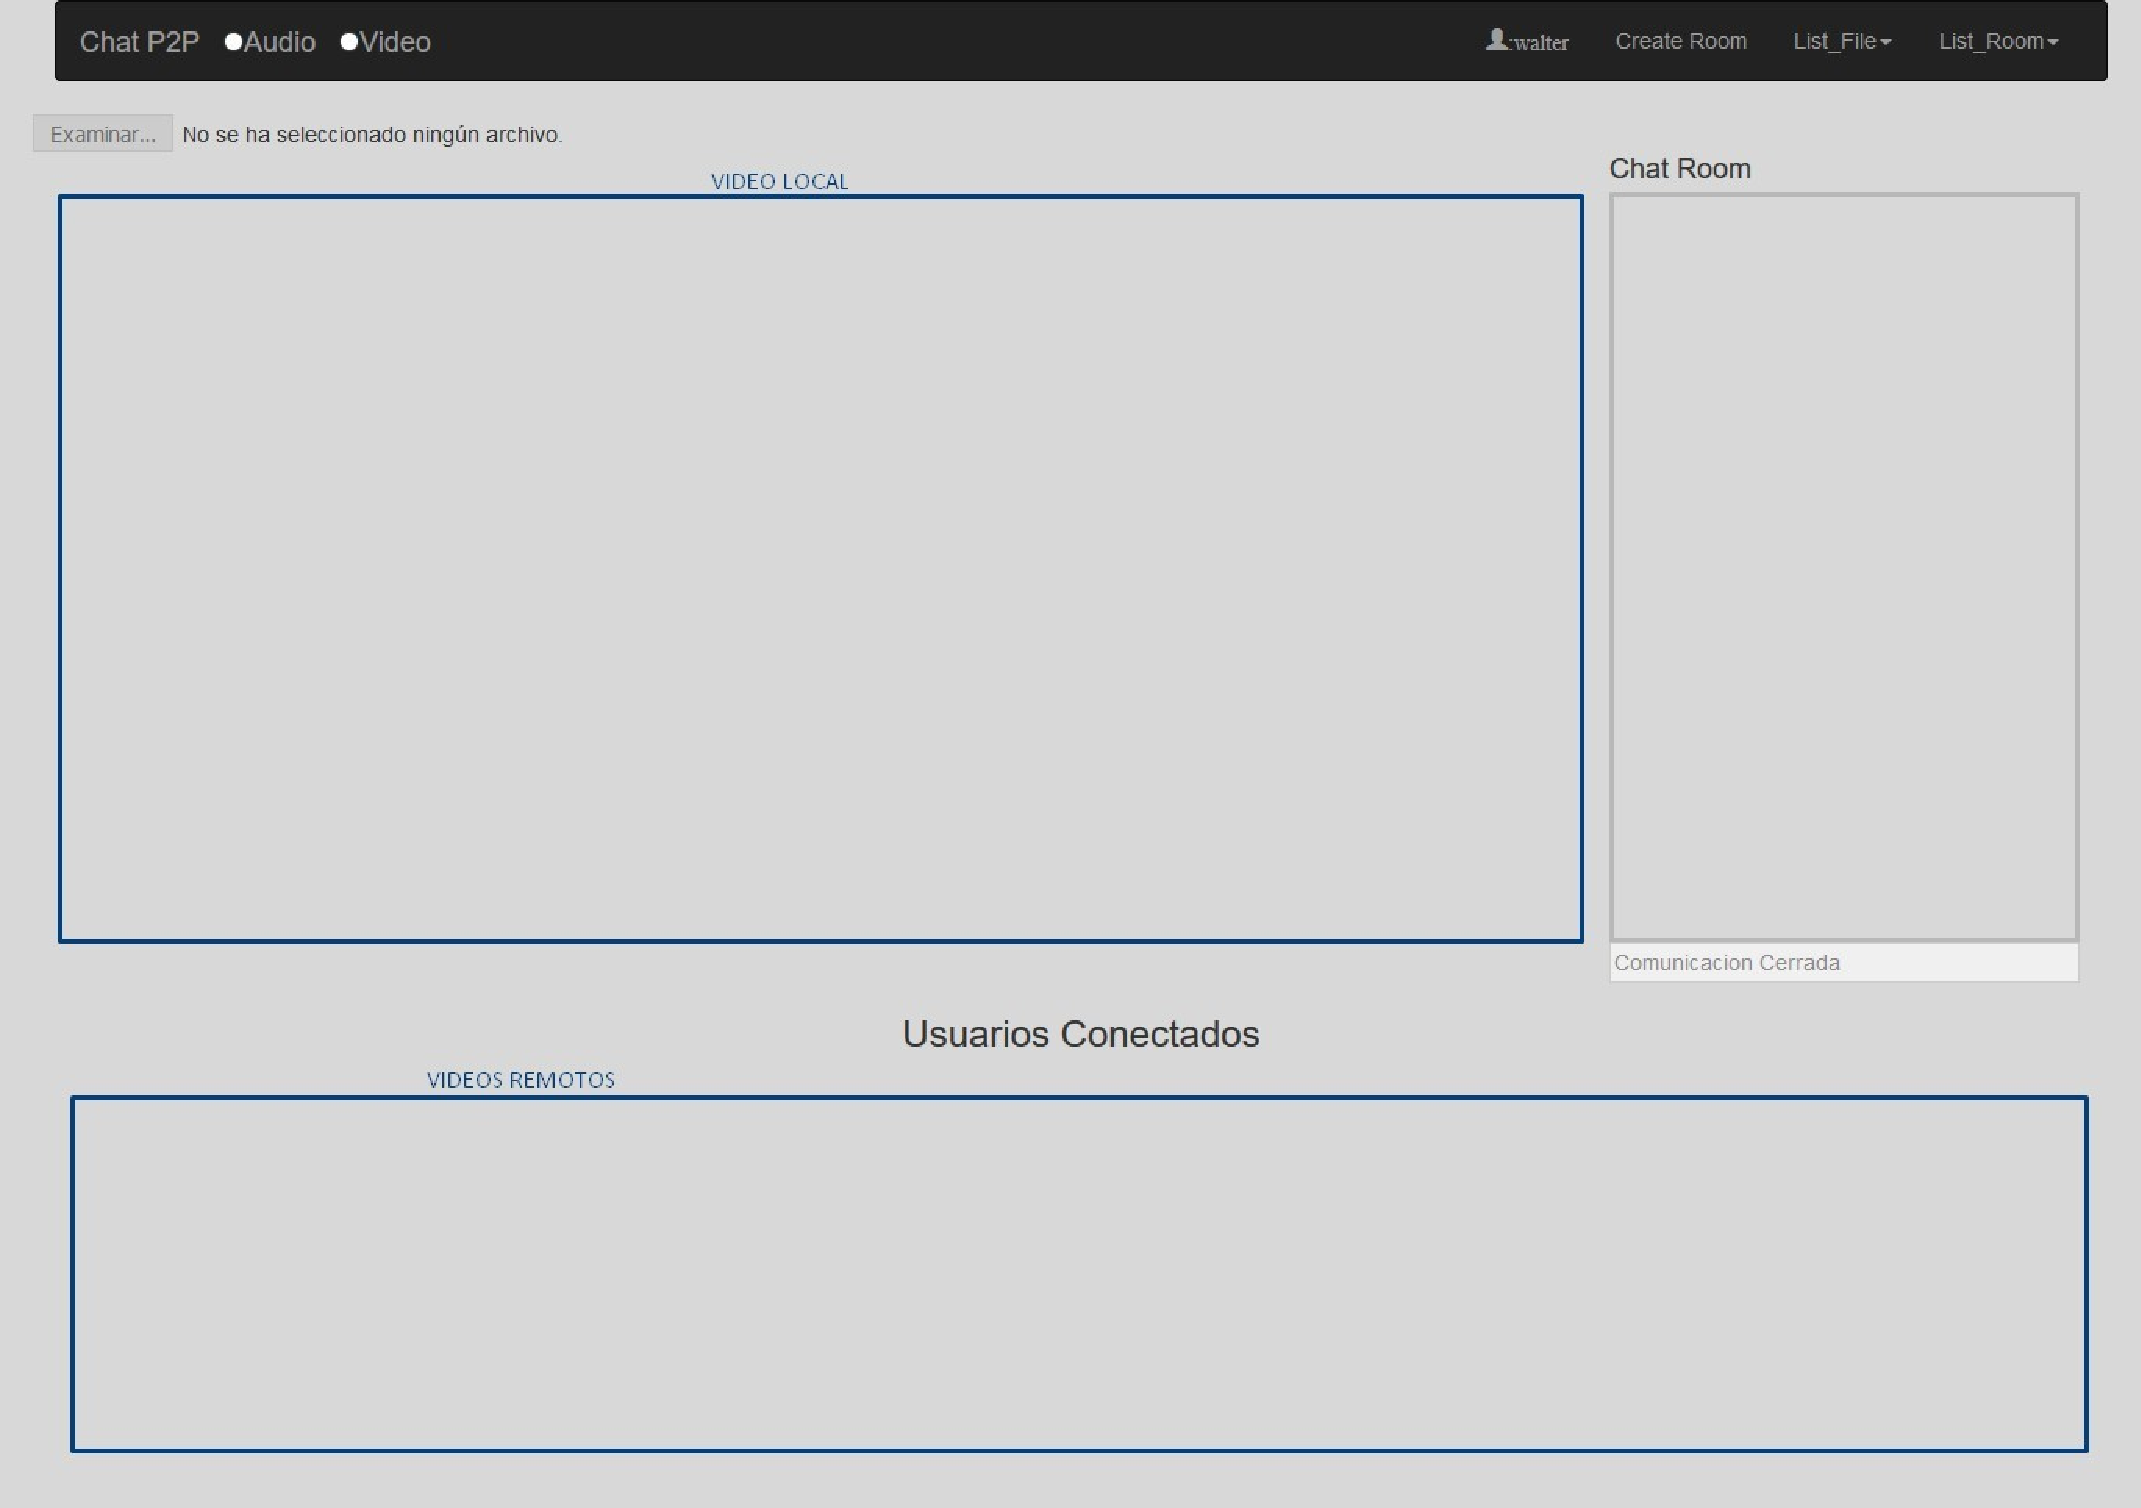
\includegraphics[width=0.6\linewidth]{Figures/esqueletoPractica}
\decoRule
\caption[An Electron]{ComunnicacionWebRTC (artist's impression).}
\label{fig:Conexcion_finish}
\end{figure}
\\\textbf{Conectividad}
\\El usuario se conecta a la direccion Ip a traves del navegador accediendo a la pagina principal de la practica la cual pedira el nombre que el usuario utilizara durante su estancia en la web. 
\\Realizamos la conexion al servidor a traves de websocket y enviamos un mensaje 'infoRoom' al servidor para obtener la lista de salas creadas y recibira el mensaje 'ReplayInfoRoom' con la informacion solicitada.
\begin{lstlisting}[
frame=single,
commentstyle=\color{CadetBlue},
captionpos=b,
caption=Incluir elementos multimedia remotos l.]
 // Connect to signalling server
 var socket = io.connect("http://localhost:8181");
 /* pedimos informacion sobre las salas que estan disponibles */
 socket.emit('infoRoom',name);
 /* anadimos las salas que estan disponibles  */
 socket.on('ReplayInfoRoom',function(listRoom){
  for(var i = 0; i < listRoom.length; i++) {
   var room = listRoom[i];
   /* Anadimos en nuestro div los usuarios para crear una coneccion  */
   if(room.state != 'block'){
    $('#listRoom').append('<li><a id='+room.name+'>'+room.name+'</a></li>');
    $('#'+room.name).click(function(){
      nameRoom = $(this).text();
      attachmentElements();
    });
  }else{
   $('#listRoom').append('<li><a id='+room.name+'>'+room.name+':lleno'+'</a></li>');
  }
 }	
});
\end{lstlisting}
Tras esta primera conexion el usuario pasa a seleccionar los elementos que desea compartir y elige el modo en el que desea realizar la conexion ya que dispone unirse a una sala ya existente o crear nueva.
\\En cualquier caso se ejecuta la funcion 'User ItemMedia' en la cual reliazamos la llamada a 'GetUserMedia' que recibe como parametros los elementos para compartir,la funcion que se encarga de conectar los elementos y la funcion que se encarga de posibles errores.en la que envía un mensaje 'stablishConnect ' al servidor el cual contesta con un mensaje 'CreateStream'. Con este mensaje el usuario se conecta a los servicios seleccionados anteriormente a traves de  'GetUserMedia' (4.1 Point).
\begin{lstlisting}[
frame=single,
commentstyle=\color{CadetBlue},
captionpos=b,
caption=Incluir elementos multimedia remotos l.]
 function User_ItemMedia(){
  navigator.getUserMedia(items,connect_items,error_items);
 }
 \end{lstlisting}
 Dentro de la funcion 'connect items' evaluamos el tipo de navegador utilizado para seleccionar la mejor forma de presentar el video local. Finalmente, enviamos el mensaje  'stablish connection'. 
 \begin{lstlisting}[
frame=single,
commentstyle=\color{CadetBlue},
captionpos=b,
caption=Incluir elementos multimedia remotos l.]
 function connect_items(stream){
  streaming = stream;
  if(webrtcDetectedBrowser == 'firefox'){
   localvideo.mozSrcObject = stream;
  }else{
   localvideo.srcObject = stream;
  }
  socket.emit('stablish_connection',name,nameRoom);
}
\end{lstlisting}
Cuando el servidor procesa el mensaje nos envia un mensaje 'CreateStream' con el id que el usuario utilizara. 
\begin{lstlisting}[
frame=single,
commentstyle=\color{CadetBlue},
captionpos=b,
caption=Incluir elementos multimedia remotos l.]
 socket.on('CreateStream',function(id){
  my_id = id;
 });
\end{lstlisting}
Cuando se conecta un nuevo usuario se envia el mensaje 'New Joined' con el id del nuevo usuario a los  existentes en sala  quienes comienzan el proceso de señalizacion que se compene de tres etapas : oferta,respuesta y icecandidate.
\begin{lstlisting}[
frame=single,
commentstyle=\color{CadetBlue},
captionpos=b,
caption=Incluir elementos multimedia remotos l.]
 socket.on('New_Joined',function(id){
  id_newUser = id;
  create_connection(id_newUser);
 });
\end{lstlisting}
\textbf{\textit{Oferta}} 
\\La funcion 'create connection' se encarga de crear los distintos elementos necesarios en la creacion de la oferta. Primero definimos la variable con la configuracion necesario para emplear el protocolo ICE del que depende RTCPeerConnection.
\begin{lstlisting}[
frame=single,
commentstyle=\color{CadetBlue},
captionpos=b,
caption=Incluir elementos multimedia remotos l.]
 var pc_config = {'iceServers': [{'url': 'stun:stun.l.google.com:19302'}]};
 var pc = new RTCPeerConnection(pc_config,{});
 var num_user = 'user_'+ list_user.length;
 new_remote(num_user);
\end{lstlisting}
A continuacion creamos una instancia de RTCPeerConnection y lo guardamos en la variable 'pc'. A traves de esta variable definimos una serie de eventos, con uno de ellos atamos el video local a la conexion con 'pc.addStream()' y el remoto a traves 'pc.onaddstream' en el que vinculamos el flujo de video con su correspondinte etiqueta.
\begin{lstlisting}[
frame=single,
commentstyle=\color{CadetBlue},
captionpos=b,
caption=Incluir elementos multimedia remotos l.]
 /* video local */
 pc.addStream(streaming);

 /*  video remoto*/
 pc.onaddstream = function(event){
  var video = document.querySelector('#'+num_user);
  video.mozSrcObject = event.stream;
  video.play();
 };
\end{lstlisting}
Pasamos a definir el canal de comunicacion de datos a traves del metodo 'pc.createDataChannel'  al que le pasamos el nombre que recibe el canal y definimos los eventos necesarios para trabajar los mensajes entre los cliente.
\begin{lstlisting}[
frame=single,
commentstyle=\color{CadetBlue},
captionpos=b,
caption=Incluir elementos multimedia remotos l.]
 /* canal de datos */
 var sendChannel = pc.createDataChannel("sendDataChannel",{reliable: true})
 /* guardamos el canal */
 list_send.push(sendChannel);	
 /* eventos manejo de datos */
 sendChannel.onopen = ChannelOpen;
 sendChannel.onclose = ChannelClose;
 sendChannel.onmessage = ChannelReceive;
\end{lstlisting}
Finalmente, definimos el metodo 'pc.createOffer()' en el que guardamos la descripcion de sesion con el metodo 'pc.setLocalDescription(sessionDescription)' y enviamos un mensaje 'message' donde el cuerpo del mensaje es la oferta generada.
\begin{lstlisting}[
frame=single,
commentstyle=\color{CadetBlue},
captionpos=b,
caption=Incluir elementos multimedia remotos l.]
 pc.createOffer(function(sessionDescription){
  //guardamos esto en nuestra session
  pc.setLocalDescription(sessionDescription);
  //enviamos nuestra descripcion al nuevo usuario
  var message = create_msg(my_id,id_newUser,sessionDescription);
  socket.emit('message',message);
 },function(err){console.log(err);},{});
\end{lstlisting}
Pasamos a generar la oferta con 'createoffer'  en el que se incluye la descripción de la sesión Tras realizar este proceso se añade la informacion
\begin{lstlisting}[
frame=single,
commentstyle=\color{CadetBlue},
captionpos=b,
caption=Incluir elementos multimedia remotos l.]
 pc.onicecandidate = SendICecandidate;
 //enviamos la oferta al nuevo usuario
 list_user.push({id:id_newUser,peer:pc,data:sendChannel});
\end{lstlisting}
\textbf{\textit{Answer}}
\\El nuevo cliente al recibir el mensaje 'message' y evaluamos el subtipo de mensaje ya que a traves de este tipo de mensaje recibimos los distintos elementos de la señalizacion. El proceso que se sigue es similiar al que realizamos en la creacion de oferta excepto porque se definen otros elementos con la informacion que recibida en el mensaje.
\\Primero , con la informacion recibida  generamos una descripcion de session con la API RTCSessionDescription al que le pasamos la informacion y lo guardamos como informacion remota .
\begin{lstlisting}[
frame=single,
commentstyle=\color{CadetBlue},
captionpos=b,
caption=Incluir elementos multimedia remotos l.]
 /*session remota  */
 pc.setRemoteDescription(new RTCSessionDescription(message.message));
\end{lstlisting}
La creacion del canal de datos lo realiza el cliente quien envia la oferta por lo que en el receptor solo creamos la instancia del canal para recibir mensajes ya que solo se puede crear un canal por cada conexion existente entre dos usuarios.
\begin{lstlisting}[
frame=single,
commentstyle=\color{CadetBlue},
captionpos=b,
caption=Incluir elementos multimedia remotos l.]
 pc.ondatachannel = function(event){
  list_send.push(event.channel);
  var receiveChannel = event.channel;
  /* evento de recepcion */
  receiveChannel.onmessage = ChannelReceive;
  receiveChannel.onopen = ChannelOpen;
  receiveChannel.onclose = ChannelClose;
 }
 \end{lstlisting}
 icen candidate
\begin{lstlisting}[
frame=single,
commentstyle=\color{CadetBlue},
captionpos=b,
caption=Incluir elementos multimedia remotos l.]
 pc.onicecandidate = function (event){
  if(event.candidate){
   var ice = { type: 'iceCandidate',
     label: event.candidate.sdpMLineIndex,
     id: event.candidate.sdpMid,
     candidate: event.candidate.candidate
  };
  var message = create_msg(my_id,message.id_origen,ice);
  socket.emit('message',message);
}
\end{lstlisting}
Finalmente, pasamos a crear la respuesta a la oferta en la cual guardamos la descripcion de session del nodo como lo realizamos en la oferta y enviamos la informacion para que el usuario conosca la informacion de sesion.
\begin{lstlisting}[
frame=single,
commentstyle=\color{CadetBlue},
captionpos=b,
caption=Incluir elementos multimedia remotos l.]
 pc.createAnswer(function(sessionDescription){
  pc.setLocalDescription(sessionDescription);
  var msg = create_msg(my_id,message.id_origen,sessionDescription);
  socket.emit('message',msg);
 },function(err){console.log(err);},{});
\end{lstlisting}
\textbf{\textit{Envió de Archivos/ texto }}
\\Se ha incorporado la posibilidad de envió de ficheros entre los clientes de la sala. Para llevar a cabo el usuario dispone de un input que permite seleccionar el fichero  y tras se ejecuta el funcionamiento de lectura Primero leemos  el archivo que se ha seleccionado  para ello utilizamos API File (point 5) y seleccionamos el modo de lectura 'readAsArrayBuffer(file)'. Una vez el archivo se ha leído completamente , a través del método 'onload', convertimos el resultado en caracteres para ser enviados al resto de usuarios.
\begin{lstlisting}[
frame=single,
commentstyle=\color{CadetBlue},
captionpos=b,
caption=Incluir elementos multimedia remotos l.]
 function processFiles(file){
  var files = file[0];
  type = files.type;
  name_fich = files.name;
  var reader = new FileReader();
  reader.onload = function (e) {
   var data_file = reader.result;
   data_encript = arrayBufferToBase64(data_file);
   send_chucky();
  };
  reader.readAsArrayBuffer(files);
 }
\end{lstlisting}
El envió de los datos lo realizamos en pequeños fragmentos ya que no sabemos la longitud del archivo y con el fin de no saturar el canal lo realizamos de esta forma. Establecemos una longitud fija para los fragmentos  y se comprueba en cada envió si nos encontramos ante el ultimo fragmento en cuyo caso enviamos información adicional archivo(nameFile,typeFile) y el un 'boolean' a true para indicar que es el ultimo fragmento.
Para  enviar  los fragmentos nos apoyamos en el evento time de JavaScript 'setTimeout(sendChuncky,time)'
\begin{lstlisting}[
frame=single,
commentstyle=\color{CadetBlue},
captionpos=b,
caption=Incluir elementos multimedia remotos l.]
 function send_chucky(){
  var last = false;
  fin = inicio + size_data;
  if(fin < data_encript.length){
   var data = JSON.stringify({info:'file',data:data_encript.slice(inicio, fin)});
   for(var i=0;i<list_send.length;i++){
    var user = list_send[i];
    user.send(data);
   }
   inicio = fin;
   setTimeout(send_chucky, 100);
  }else{
   last = true;
   var more_info ={type:type,name:name_fich};
   var data = JSON.stringify({info:'file',end:last,data:data_encript.slice(inicio, data_encript.length),more:more_info});
   for(var i=0;i<list_send.length;i++){
    var user = list_send[i];
    user.send(data);
   }
   inicio = 0;
  }
}
\end{lstlisting}
\subsubsection{Servidor de señalización}
Como se ha visto hasta el momento los usuarios intercambian informacion previa al establecimiento de conexion para ello es necesesario diseñar un servidor de señalizacion.Para ello  utilizamos NodeJS que a traves de las bibliotecas de las que dispone permite una creacion rapida . 
\\El siguiente paso es definir socket.IO como metodo de conexion a traves de npm se consigue instalarlo.
\begin{lstlisting}[
frame=single,
commentstyle=\color{CadetBlue},
captionpos=b,
caption=Incluir elementos multimedia remotos l.]
/* creacion server */
 var app = http.createServer(function (req, res) {
  file.serve(req, res);
 }).listen(8181);
 
/* instancia  websockets*/
 var io = require('socket.io').listen(app);
\end{lstlisting}
Las funcionalidades que el servidor necesita cubrir lo dividimos en dos grupos aquellas peticiones que tienen que ver con la conexion inicial de los clientes y los del proceso de señalizacion.
\\
\\\textit{\textbf{Conexion inicial de los clientes}}
\\Cuando un usuario se conecta el servidor recibe un mensaje  'infoRoom' y el servidor contesta con un mensaje 'ReplayInfoRoom' con la lista de salas disponibles en ese momento.
\begin{lstlisting}[
frame=single,
commentstyle=\color{CadetBlue},
captionpos=b,
caption=Incluir elementos multimedia remotos l.]
 socket.on('infoRoom',function(name) {
  socket.emit('ReplayInfoRoom',listRooom);
 });
\end{lstlisting}
Cuando el usuario seleccion una sala nueva o una ya existente este envia un mensaje 'stablish connection' al servidor con el nombre del usuario y el de la sala.\\El servidor con esta informacion evalua la existencia de la sala ya que en caso de no existir la crea y pasa a comprobar el numero de usuarios dentro de la sala para no exceder el maximo.
\\Si la sala no esta completa el servidor envía un mensaje 'CreateStream' para informar al usuario que tiene permisos para acceder a la sala y un mensaje' NewJoined' a todos los usuarios menos al nuevo.
\begin{lstlisting}[
frame=single,
commentstyle=\color{CadetBlue},
captionpos=b,
caption=Incluir elementos multimedia remotos l.]
 socket.on('stablish_connection',function(name,room){
  /*comprobamos la existencua de la sala */
  if(!getRoom(room)){
    setRoom(room,'');
  };
  /* comprobamos el numero de usuarios */
  var numClients = io.sockets.clients(room).length;
  if(numClients < 3){
   socket.username = name;
   socket.room =room;
   socket.join(room);
   socket.emit('CreateStream',socket.id);
   socket.broadcast.to(room).emit('New_Joined',socket.id);
  }else{
   socket.emit('RejectStream',socket.id);
  }
 });
\end{lstlisting}
\textbf{\textit{Mensaje de Señalización}}
\\Los mensajes que viajan en este proceso reciben el nombre  'message' y tienen la siguiente estructua.
\\dibujo de la estrcutur
\\Donde el 'id dest' lo consulta el servidor para poder enviar el mensaje al cliente correcto el resto de la informacion es utilizada por el cliente que reciba el mensaje.
\begin{lstlisting}[
frame=single,
commentstyle=\color{CadetBlue},
captionpos=b,
caption=Incluir elementos multimedia remotos l.]
 socket.on('message',function(message,room){
  io.sockets.socket(message.id_dest).emit('message', message);
 });
\end{lstlisting}